% USEFUL LINKS:
% -------------
%
% - UiO LaTeX guides:          https://www.mn.uio.no/ifi/tjenester/it/hjelp/latex/
% - Mathematics:               https://en.wikibooks.org/wiki/LaTeX/Mathematics
% - Physics:                   https://ctan.uib.no/macros/latex/contrib/physics/physics.pdf
% - Basics of Tikz:            https://en.wikibooks.org/wiki/LaTeX/PGF/Tikz
% - All the colors!            https://en.wikibooks.org/wiki/LaTeX/Colors
% - How to make tables:        https://en.wikibooks.org/wiki/LaTeX/Tables
% - Code listing styles:       https://en.wikibooks.org/wiki/LaTeX/Source_Code_Listings
% - \includegraphics           https://en.wikibooks.org/wiki/LaTeX/Importing_Graphics
% - Learn more about figures:  https://en.wikibooks.org/wiki/LaTeX/Floats,_Figures_and_Captions
% - Automagic bibliography:    https://en.wikibooks.org/wiki/LaTeX/Bibliography_Management  (this one is kinda difficult the first time)
%
%                              (This document is of class "revtex4-1", the REVTeX Guide explains how the class works)
%   REVTeX Guide:              http://www.physics.csbsju.edu/370/papers/Journal_Style_Manuals/auguide4-1.pdf
%
%
% COMPILING THE .pdf FILE IN THE LINUX TERMINAL
% ---------------------------------------------
%
% [terminal]$ pdflatex report_example.tex
%
% Run the command twice, always.
%
% When using references, footnotes, etc. you should run the following chain of commands:
%
% [terminal]$ pdflatex report_example.tex
% [terminal]$ bibtex report_example
% [terminal]$ pdflatex report_example.tex
% [terminal]$ pdflatex report_example.tex
%
% This series of commands can of course be gathered into a single-line command:
% [terminal]$ pdflatex report_example.tex && bibtex report_example.aux && pdflatex report_example.tex && pdflatex report_example.tex
%
% ----------------------------------------------------



% \documentclass[english,notitlepage,reprint,nofootinbib]{revtex4-2}  % defines the basic parameters of the document
\documentclass[english,notitlepage,reprint,nofootinbib]{revtex4-2}  % defines the basic parameters of the document
% If you want a single-column, remove "reprint"

% Allows special characters (including æøå)
\usepackage[utf8]{inputenc}
% \usepackage[english]{babel}

% Note that you may need to download some of these packages manually, it depends on your setup.
% It may be usefult to download TeXMaker, because it includes a large library of the most common packages.

\usepackage{physics,amssymb}  % mathematical symbols (physics imports amsmath)
\include{amsmath}
\usepackage{graphicx}         % include graphics such as plots
\usepackage{xcolor}           % set colors
\usepackage{hyperref}         % automagic cross-referencing
\usepackage{listings}         % display code
\usepackage{subfigure}        % imports a lot of cool and useful figure commands
% \usepackage{float}
%\usepackage[section]{placeins}
\usepackage{algorithm}
\usepackage[noend]{algpseudocode}
\usepackage{subfigure}
\usepackage{tikz}
\usetikzlibrary{quantikz}
% defines the color of hyperref objects
% Blending two colors:  blue!80!black  =  80% blue and 20% black
\hypersetup{ % this is just my personal choice, feel free to change things
    colorlinks,
    linkcolor={red!50!black},
    citecolor={blue!50!black},
    urlcolor={blue!80!black}}


% ===========================================


\begin{document}

\title{FYS4150 - Project 1}  % self-explanatory
\author{Isak Cecil Onsager Rukan} % self-explanatory
\date{\today}                             % self-explanatory
\noaffiliation                            % ignore this, but keep it.
\maketitle
The one-dimensional Poisson can be written as 
\begin{align}
    -\frac{d^2u}{dx^2} = f(x),  \label{eq:Poisson}
\end{align}
where $f(x)$ is some known function. In this project we let \(x\in[0,1]\) and
\begin{align}
    f(x) = 100e^{-10x}, \label{eq:f_x}
\end{align}
together with the following boundary conditions
\begin{align}
    u(0)=0, \quad u(1)=0. \label{eq:boundary_condition}
\end{align}
\section{Problem 1}
% We will show that an analytic solution to \eqref{eq:Poisson} with \(f(x)\) given in \eqref{eq:f_x} is:
% \begin{align}
%     u(x) = 1 - (1-e^{-10})x - e^{-10x}.
% \end{align} 
Let $v(x)=d/dx u(x)$. Integrating \eqref{eq:Poisson} leads to 
\begin{align}
    -v(x) &= 100\int dxe^{-10x}
    \notag \\
    &= -10e^{-10x} + C,
\end{align}
which means that 
\begin{align}
    u(x) &= \int v(x) 
    \notag \\
    &= -e^{-10x} - Cx + D.
\end{align}
Here $C$ and $D$ are some constants which are determined by the boundary conditions in \eqref{eq:boundary_condition}. Concretely, \(u(0)=0\) leads to $D=1$ and then \(u(1)=0\) sets \(C=-(1-e^{-10})\). Hence,
\begin{align}
    u(x) = 1 - (1 - e^{-10x})x - e^{-10x}.  \label{eq:u_x}
\end{align}
\section{Problem 2}
Using \href{https://github.com/isakrukan/FYS4150/blob/main/Project1/Code/problem2.cpp}{problem2.cpp} we compute $u(x)$ numerically for $N=10^4$ points. The result is written to \href{https://github.com/isakrukan/FYS4150/blob/main/Project1/Code/problem2.txt}{problem2.txt} and Fig. \ref{fig:u_x} is made in \href{https://github.com/isakrukan/FYS4150/blob/main/Project1/Code/problem2.py}{problem2.py}.
\begin{figure}[h!]
    \centering
    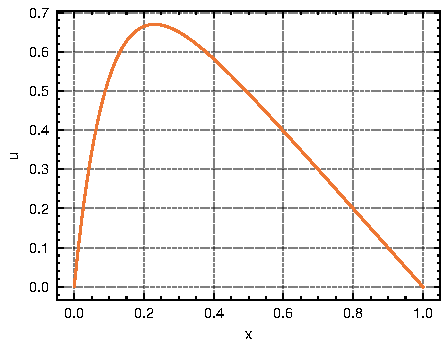
\includegraphics{Figs/problem2.pdf}
    \caption{Eq. \eqref{eq:u_x} using $N=10^4$ points.}
    \label{fig:u_x}
\end{figure}

\section{Problem 3}
The second derivative of $u(x)$, appearing on the R.H. side of \eqref{eq:Poisson} may be written as
\begin{align}
    \frac{d^2}{dx^2}u(x) = \lim_{h\rightarrow 0} \frac{u(x+h) -2u(x) + u(x-h)}{h^2}.    \label{eq:second_order_derivative}
\end{align}
To approximate this limit numerically, let $h$ be small and $\vec{x}$ be an array of $n$ points equispaced from zero to one. Eq. \eqref{eq:second_order_derivative} can then be approximated up to order $\mathcal{O}(h^2)$:
\begin{align}
    \frac{d^2}{dx^2}u(x)\vert_{x_i} = \frac{u(x_{i+1}) - 2u(x_i) + u(x_{i-1})}{h^2} + \mathcal{O}(h^2).  \label{eq:discretized_version_second_derivative}
\end{align}   
Since, according to \eqref{eq:Poisson}, the second derivative of $u(x)$ equals $-f(x)$, we can write \eqref{eq:discretized_version_second_derivative} as  
\begin{align}
    -h^2f(x_i) = \frac{u(x_{i+1}) - 2u(x_i) + u(x_{i-1})}{h^2} + \mathcal{O}(h^2). \label{eq:Poisson_disc}
\end{align}

\section{Problem 4}
Let $\vec{v} = (v_1,...,v_{n})$ be a vector whose $i$-th component is thought of as representing the numerical implementation (so ignoring the order $\mathcal{O}(h^2)$) of $u_{i+1}$.
Eq. \eqref{eq:Poisson_disc} can then be written as 
\begin{align}
    -v_{i-1} + 2v_{i} - v_{i+1} = h^2f(x_i).    \label{eq:numerical_v}
\end{align}
Further, 
let $\vec{g}$ be the vector of length \(n\), given by componentwise as 
\begin{align}
    \vec{g}_{i} = h^2f(x_{i+1}), i = 2, ..., n-1, 
\end{align}
and \(\vec{g}_{1} = h^2f(x_{1}) + u(0)\), \(\vec{g}_{n} = h^2f(x_{n}) + u(1)\). Then, if we let $A$ be the \(n\times n\)-matrix given by
\begin{align}
    A = \begin{pmatrix}
        2 & -1 & 0 & \cdots & 0 \\
        -1 & 2 & -1 & \ddots & \vdots \\
        0 & -1 & 2 & \ddots & 0 \\
        \vdots & \ddots & \ddots & \ddots & -1 \\
        0 & \cdots & 0 & -1 & 2
    \end{pmatrix},
\end{align}
we can represent \eqref{eq:numerical_v} as 
\begin{align}
    A\vec{v} = \vec{g}. \label{eq:as_matrix_multiplication}
\end{align}
To see that this explicitly, multiply the matrix $A$ with $\vec{v}$, which gives $A\vec{v}$ componentwise as
\begin{align}
    (A\vec{v})_{i} &= -v_{i-1} + 2v_{i} - v_{i+1}, \quad i = 2, ..., n-1.
\end{align}
For \(i=0\): \((A\vec{v})_{0} = 2v_{0} - v_{1}\), and \(i=n\): \((A\vec{v})_{n} = -v{n-1} + 2v_{n}\).



\section{Problem 5}
The vector $\vec{v}$ does not contain the boundary points corresponding to $x_{0}=0$ and $x_{N-1}=1$. Let the vector $\vec{v}^*$ be given by 
\begin{align}
    \vec{v}^* = (u(0), \vec{v}, u(1)).
\end{align}
Then, clearly, \(\vec{v}^*\) is a vector of length $n$ and when solving \eqref{eq:as_matrix_multiplication} we will obtain $\vec{v}$, which is \(\vec{v}^*\) excluding its first and last component.

\section{Problem 6}
Consider now $A$ as a general tridiagonal matrix with vectors $\vec{a}, \ \vec{b}$ and \(\vec{c}\) representing the subdiagonal, main diagonal and superdiagonal, respectively. When solving \eqref{eq:as_matrix_multiplication} we may then use a number of row operations on $A$, such that it turns into a matrix $\tilde{A}$ with all entries below the diagonal equal to zero. These row operations naturally alters the $\vec{\tilde{g}}$ on R.H. side of \eqref{eq:as_matrix_multiplication} into a vector $\tilde{g}$, at which point the solution to \eqref{eq:as_matrix_multiplication} can then be simply read of by multiplying out $\tilde{A}\vec{v} = \vec{\tilde{g}}$.

Let $R_{i}$ denote the $i$-th row of \eqref{eq:as_matrix_multiplication}. In the following, when writing $\overset{aR_i-b R_j}{\rightarrow}$, we mean the row operation of subtracting $b$ times row \(j\) from \(a\) times row \(i\). When applying a row operation to the $i$-th row, we write \(\tilde{b}_{j}\) and \(\tilde{g}_j\) as the resulting new \(j\)-th component of the vector \(\vec{b}\) and \(\vec{g}\), respectively. We have:
\begin{widetext}
\begin{align}
    &\left[\begin{array}{cccccc|c}
        R_1: & b_1 & c_1 & 0 & \cdots & 0  & g_1\\
        R_2: & a_{2} & b_2 & c_2 & \ddots & \vdots  & g_2\\
        R_3: & 0 & a_{3} & b_3 & \ddots & 0  & g_3\\
        \ & \vdots & \ddots & \ddots & \ddots & c_{n-1}  & \vdots\\
        R_{n}: & 0 & \cdots & 0 & a_{n-1} & b_{n} & g_{n}
    \end{array}\right]
    \notag \\
    \overset{R_2 - a_2/b_1R_1}{\longrightarrow} 
    &\left[\begin{array}{cccccc|c}
        R_1: & b_1 & c_1 & 0 & \cdots & 0  & g_1\\
        R_2: & 0 & b_2-a_2\frac{c_1}{b_1} & c_2 & \ddots & \vdots  & g_2-g_1\frac{a_2}{b_1}\\
        R_3: & 0 & a_{3} & b_3 & \ddots & 0  & g_3\\
        \ & \vdots & \ddots & \ddots & \ddots & c_{n-1}  & \vdots\\
        R_{n} & 0 & \cdots & 0 & a_{n-1} & b_{n} & g_{n}
    \end{array}\right]
    \notag \\
    \overset{R_3 - a_3/\tilde{b}_2R_2}{\longrightarrow} 
    &\left[\begin{array}{cccccc|c}
        R_1: & b_1 & c_1 & 0 & \cdots & 0  & g_1\\
        R_2: & 0 & \tilde{b}_2 & c_2 & \ddots & \vdots  & \tilde{g}_2\\
        R_3: & 0 & 0 & b_3 - a_{3}\frac{c_2}{\tilde{b}_2} & \ddots & 0  & g_3 - g_2\frac{a_3}{\tilde{b}_1}\\
        \ & \vdots & \ddots & \ddots & \ddots & c_{n-1}  & \vdots\\
        R_{n} & 0 & \cdots & 0 & a_{n-1} & b_{n} & g_{n}
    \end{array}\right]
\end{align}
Continuing in this way we obtain 
\begin{subequations}    \label{eq:tilde_b_ntilde_g}
\begin{align}
    \tilde{b}_{j} = b_{j} - a_{j}\frac{c_{j-1}}{b_{j-1}}, \quad j=2,..., n,   \label{eq:tilde_b}\\ 
    \tilde{g}_{j} = g_{j} - a_{j}\frac{g_{j-1}}{b_{j-1}}, \quad j=2,..., n,   \label{eq:tilde_g}
\end{align}
\end{subequations}
with \(\tilde{b}_1 = b_1\) and \(\tilde{g}_1 = g_1\). After having performed these row operations, we can perform backward substitution from the last row:
\begin{align}
    &\left[\begin{array}{cccccc|c}
        R_1: & b_1 & c_1 & 0 & \cdots & 0  & g_1\\
        \ & \vdots & \ddots & \ddots & \ddots & 0  & \vdots \\
        R_{n-2}:   & 0 & \cdots & \tilde{b}_{n-2} & c_{n-2} & 0 & \tilde{g}_{n-2} \\
        R_{n-1}: & 0 & \cdots & 0 & \tilde{b}_{n-1} & c_{n-1} & \tilde{g}_{n-1} \\
        R_{n}: & 0 & \cdots & 0 & 0 & \tilde{b}_{n} & \tilde{g}_{n} 
    \end{array}\right]
    \notag \\
    \overset{R_{n}/\tilde{b}_{n}}{\longrightarrow} 
    &\left[\begin{array}{cccccc|c}
        R_1: & b_1 & c_1 & 0 & \cdots & 0  & g_1\\
        \ & \vdots & \ddots & \ddots & \ddots & 0  & \vdots \\
        R_{n-2}:   & 0 & \cdots & \tilde{b}_{n-2} & c_{n-2} & 0 & \tilde{g}_{n-2} \\
        R_{n-1}: & 0 & \cdots & 0 & \tilde{b}_{n-1} & c_{n-1} & \tilde{g}_{n-1} \\
        R_{n}: & 0 & \cdots & 0 & 0 & 1 & \frac{\tilde{g}_{n}}{\tilde{b}_{n}}
    \end{array}\right]
\end{align}
meaning that 
\begin{align}
    v_{n} &= \frac{\tilde{g}_{n}}{\tilde{b}_{n}}. \label{eq:last_v}
\end{align}
Then, performing the row-operation 
\begin{align}
    R_{n-1}\rightarrow (R_{n-1} - c_{n-1}R_{n})/\tilde{b}_{n-1},
\end{align}
gives 
\begin{align}
    % \overset{\frac{R_{n-1}}{\tilde{b}_{n}}-c_{n-1}R_{n}}{\longrightarrow} 
    &\left[\begin{array}{cccccc|c}
        R_1: & b_1 & c_1 & 0 & \cdots & 0  & g_1\\
        \ & \vdots & \ddots & \ddots & \ddots & 0  & \vdots \\
        R_{n-2}:   & 0 & \cdots & \tilde{b}_{n-2} & c_{n-2} & 0 & \tilde{g}_{n-2} \\
        R_{n-1}: & 0 & \cdots & 0 & 1 & 0 & \frac{\tilde{g}_{n-1} - c_{n-1}v_{n}}{\tilde{b}_{n-1}} \\
        R_{n}: & 0 & \cdots & 0 & 0 & 1 & v_{n}
    \end{array}\right]
    \notag \\
    \overset{\frac{R_{n-2}}{\tilde{b}_{n-2}}-\frac{c_n-2}{\tilde{b}_{n-2}}R_{n-1}}{\longrightarrow} 
    &\left[\begin{array}{cccccc|c}
        R_1: & b_1 & c_1 & 0 & \cdots & 0  & g_1\\
        \ & \vdots & \ddots & \ddots & \ddots & 0  & \vdots \\
        R_{n-2}:   & 0 & \cdots & 1 & 0 & 0 & \frac{\tilde{g}_{n-2} - c_{n-2}v_{n-1}}{\tilde{b}_{n-2}} \\
        R_{n-1}: & 0 & \cdots & 0 & 1 & 0 & v_{n-1} \\
        R_{n}: & 0 & \cdots & 0 & 0 & 1 & v_{n}
    \end{array}\right],
\end{align}
and so on, which leads to  
\begin{align}
    v_{i}   &= \frac{\tilde{g}_{i}-c_{i}v_{i+1}}{\tilde{b}_{i}}, \quad i=1, ..., n-1.   \label{eq:v_i}
\end{align}
\end{widetext}

Both \eqref{eq:tilde_b} and \eqref{eq:tilde_g} requires \(3\) floating-point operations (FLOPs) each, and hence implementing \eqref{eq:tilde_b_ntilde_g} takes a total of \(6*(n-1)\) FLOPs. Eq. \eqref{eq:last_v} takes one FLOP, while \eqref{eq:v_i} takes \(3*(n-1)\) FLOPs. Hence, the complete algorithm for obtaining \(\vec{v}\) requires \({6*(n-1) + 3*(n-1) + 1= 9n-8=\mathcal{O}(n)}\) FLOPs.

\section{Problem 7}


\onecolumngrid
% \bibliographystyle{apalike}
\bibliographystyle{unsrt}
\bibliography{ref}


\end{document}